\begin{figure}[H]
  \centering
  \begin{tabular}{ccc}
    \begin{minipage}[t]{0.2\hsize}
      \centering
      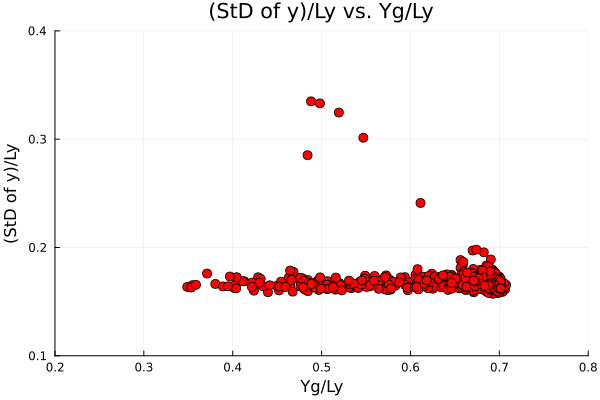
\includegraphics[width=\textwidth]{image/g0_cycle/2023-12-27T20:17:44.542_qrs_g0_chiinf_Ay50_rho0.4_T0.43_dT0.04_Rd0.0_Rt0.375_Ra0.4693845_g0_run4.0e7.png}
      \subcaption{Ra0.469}
      \label{}
    \end{minipage} &
    \begin{minipage}[t]{0.2\hsize}
      \centering
      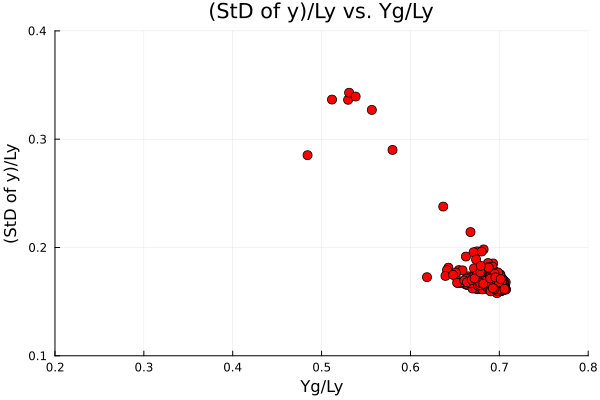
\includegraphics[width=\textwidth]{image/g0_cycle/2023-12-27T20:17:45.053_qrs_g0_chiinf_Ay50_rho0.4_T0.43_dT0.04_Rd0.0_Rt0.375_Ra0.938769_g0_run4.0e7.png}
      \subcaption{Ra0.938}
      \label{}
    \end{minipage} &
    \begin{minipage}[t]{0.2\hsize}
      \centering
      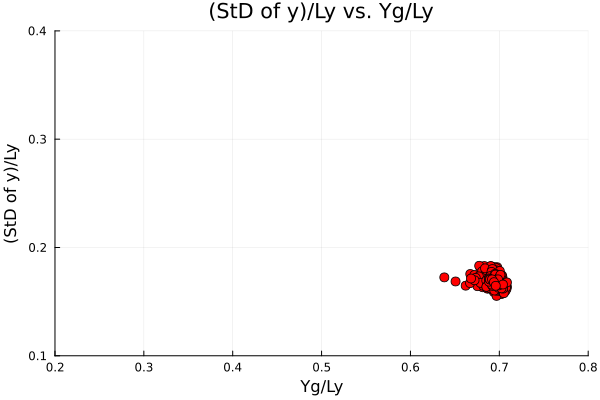
\includegraphics[width=\textwidth]{image/g0_cycle/2023-12-27T20:17:45.121_qrs_g0_chiinf_Ay50_rho0.4_T0.43_dT0.04_Rd0.0_Rt0.375_Ra1.4081535_g0_run4.0e7.png}
      \subcaption{Ra1.408}
      \label{}
    \end{minipage} 
  \end{tabular}
  \caption{$t_i = 0 , t_f = 2.0 \times 10^5, t\sqrt{\epsilon/m{\sigma}^2} = 200$ごとにプロット.}
  \label{}
\end{figure}